% answers.tex —— 2012 年·陕西卷·理科 · 参考答案与详细解析片段
% 由 tools/generate_projects.py 依来源总账自 2012/2012_数学真题_陕西理_试题.md + 2012/2012_数学真题_陕西理_解析正文.md + 2012/2012_数学真题_陕西理_答案要点.md 生成，勿手改（改源 MD 后重跑）

\begin{answer}
\gksolhead{1}{}

\textbf{题目}：

集合 $M=\{x\mid\lg x>0\}$，$N=\{x\mid x^2\leqslant4\}$，则 $M\cap N=$\mbox{（　　）}

（A）$(1,2)$；（B）$[1,2)$；（C）$(1,2]$；（D）$[1,2]$。

\Needspace{4\baselineskip}
\textbf{解析}
$M=(1,+\infty)$，$N=[-2,2]$，故 $M\cap N=(1,2]$。选 C。

\gkanswer{答案：C。}

\end{answer}
\begin{answer}
\gksolhead{2}{}

\textbf{题目}：

下列函数中，既是奇函数又是增函数的为\mbox{（　　）}

（A）$y=x+1$；（B）$y=-x^3$；（C）$y=\dfrac1x$；（D）$y=x|x|$。

\Needspace{4\baselineskip}
\textbf{解析}
（A）非奇非偶；（B）为奇函数但递减；（C）为奇函数但在定义域上不单调；（D）$f(-x)=-x|x|=-f(x)$ 且为增函数。选 D。

\gkanswer{答案：D。}

\end{answer}
\begin{answer}
\gksolhead{3}{}

\textbf{题目}：

设 $a$，$b\in\mathbf R$，$\mathrm i$ 是虚数单位，则“$ab=0$”是“复数 $a+\dfrac b{\mathrm i}$ 为纯虚数”的\mbox{（　　）}

（A）充分不必要条件；（B）必要不充分条件；（C）充分必要条件；（D）既不充分也不必要条件。

\Needspace{4\baselineskip}
\textbf{解析}
$a+\dfrac b{\mathrm i}=a-b\mathrm i$ 为纯虚数需 $a=0$ 且 $b\neq0$，这蕴含 $ab=0$；而 $ab=0$ 也可能是 $b=0$（此时为实数 $0$），故必要不充分。选 B。

\gkanswer{答案：B。}

\end{answer}
\begin{answer}
\gksolhead{4}{}

\textbf{题目}：

已知圆 $C:x^2+y^2-4x=0$，$l$ 是过点 $P(3,0)$ 的直线，则\mbox{（　　）}

（A）$l$ 与 $C$ 相交；（B）$l$ 与 $C$ 相切；（C）$l$ 与 $C$ 相离；（D）以上三个选项均有可能。

\Needspace{4\baselineskip}
\textbf{解析}
圆 $C$ 的圆心为 $(2,0)$，半径 $2$。$|PC|=1<2$，故 $P$ 在圆内，过 $P$ 的任意直线都与圆相交。选 A。

\gkanswer{答案：A。}

\end{answer}
\begin{answer}
\gksolhead{5}{}

\textbf{题目}：

如图，在空间直角坐标系中有直三棱柱 $ABC-A_1B_1C_1$，$CA=CC_1=2CB$，则直线 $BC_1$ 与直线 $AB_1$ 夹角的余弦值为\mbox{（　　）}
\nopagebreak[4]
\begin{center}% 2012 年陕西卷理科第 5 题：空间直角坐标系中的直三棱柱 ABC-A1B1C1。
% 来源 PDF：普通高考/2012/2012陕西理.pdf，第 1 页（印面 763）第 1 栏。
% 取 C(0,0,0)，A 沿 x 轴、B 沿 z 轴、C1 沿 y 轴；按原图取向作斜投影：
% x → (-0.8,-0.6)，y → (1.0,0.15)，z → (0,1)。
\begin{tikzpicture}[semithick, >=Stealth, font=\small]
  \coordinate (C)  at (0,0);
  \coordinate (A)  at (-1.6,-1.2);
  \coordinate (B)  at (0,1.4);
  \coordinate (C1) at (2.0,0.30);
  \coordinate (A1) at (0.4,-0.90);
  \coordinate (B1) at (2.0,1.70);
  % 坐标轴
  \draw[->] (0,0) -- (-2.0,-1.5) node[below] {$x$};
  \draw[->] (0,0) -- (0,1.9) node[left] {$z$};
  \draw[->] (0,0) -- (2.5,0.38) node[right] {$y$};
  % 棱柱
  \draw (C) -- (A) -- (B) -- cycle;
  \draw (A) -- (A1);
  \draw (C) -- (C1);
  \draw (B) -- (B1);
  \draw (A1) -- (B1);
  \draw (C1) -- (A1);
  \draw[dashed] (B1) -- (C1);
  \draw[dashed] (B) -- (C1);
  \draw (A) -- (B1);
  \node[below right] at (C) {$C$};
  \node[left] at (A) {$A$};
  \node[left] at (B) {$B$};
  \node[below right] at (C1) {$C_1$};
  \node[right] at (A1) {$A_1$};
  \node[above right] at (B1) {$B_1$};
\end{tikzpicture}
\end{center}
\nopagebreak[4]
（A）$\dfrac{\sqrt5}5$；（B）$\dfrac{\sqrt5}3$；（C）$\dfrac{2\sqrt5}5$；（D）$\dfrac35$。

\Needspace{4\baselineskip}
\textbf{解析}
\Needspace{5\baselineskip}
取 $C(0,0,0)$，$A(2,0,0)$，$B(0,0,1)$，$C_1(0,2,0)$，$B_1(0,2,1)$。则
\nopagebreak[4]
\[\overrightarrow{BC_1}=(0,2,-1),\qquad \overrightarrow{AB_1}=(-2,2,1),\]
\nopagebreak[4]
\[\overrightarrow{BC_1}\cdot\overrightarrow{AB_1}=0+4-1=3,\]
\nopagebreak[4]
\[|\overrightarrow{BC_1}|=\sqrt5,\qquad |\overrightarrow{AB_1}|=3.\]
故夹角的余弦值为 $\dfrac3{3\sqrt5}=\dfrac{\sqrt5}5$。选 A。

\gkanswer{答案：A。}

\end{answer}
\begin{answer}
\gksolhead{6}{}

\textbf{题目}：

从甲、乙两个城市分别随机抽取 $16$ 台自动售货机，对其销售额进行统计，统计数据用茎叶图表示（如图所示）。设甲、乙两组数据的平均数分别为 $\overline x_\text{甲}$，$\overline x_\text{乙}$，中位数分别为 $m_\text{甲}$，$m_\text{乙}$，则\mbox{（　　）}

\begin{center}
\begin{tabular}{lll}
\toprule
甲 & 茎 & 乙 \\
\midrule
$8$ $6$ $5$ & $0$ &  \\
$8$ $8$ $4$ $0$ $0$ & $1$ & $0$ $2$ $8$ \\
$7$ $5$ $2$ & $2$ & $0$ $2$ $3$ $3$ $7$ \\
$8$ $0$ $0$ & $3$ & $1$ $2$ $4$ $4$ $8$ \\
$3$ $1$ & $4$ & $2$ $3$ $8$ \\
\bottomrule
\end{tabular}
\end{center}

（A）$\overline x_\text{甲}<\overline x_\text{乙}$，$m_\text{甲}>m_\text{乙}$；（B）$\overline x_\text{甲}<\overline x_\text{乙}$，$m_\text{甲}<m_\text{乙}$；（C）$\overline x_\text{甲}>\overline x_\text{乙}$，$m_\text{甲}>m_\text{乙}$；（D）$\overline x_\text{甲}>\overline x_\text{乙}$，$m_\text{甲}<m_\text{乙}$。

\Needspace{4\baselineskip}
\textbf{解析}
甲的数据为 $5,6,8,10,10,14,18,18,22,25,27,30,30,38,41,43$，平均数为 $\dfrac{345}{16}$，中位数为 $\dfrac{18+22}2=20$。

乙的数据为 $10,12,18,20,22,23,23,27,31,32,34,34,38,42,43,48$，平均数为 $\dfrac{457}{16}$，中位数为 $\dfrac{27+31}2=29$。

故 $\overline x_\text{甲}<\overline x_\text{乙}$，$m_\text{甲}<m_\text{乙}$。选 B。

\gkanswer{答案：B。}

\end{answer}
\begin{answer}
\gksolhead{7}{}

\textbf{题目}：

设函数 $f(x)=x\mathrm e^x$，则\mbox{（　　）}

（A）$x=1$ 为 $f(x)$ 的极大值点；（B）$x=1$ 为 $f(x)$ 的极小值点；（C）$x=-1$ 为 $f(x)$ 的极大值点；（D）$x=-1$ 为 $f(x)$ 的极小值点。

\Needspace{4\baselineskip}
\textbf{解析}
$f'(x)=\mathrm e^x(1+x)$，当 $x<-1$ 时 $f'<0$，当 $x>-1$ 时 $f'>0$，故 $x=-1$ 为极小值点。选 D。

\gkanswer{答案：D。}

\end{answer}
\begin{answer}
\gksolhead{8}{}

\textbf{题目}：

两人进行乒乓球比赛，先赢 $3$ 局者获胜，决出胜负为止，则所有可能出现的情形（各人输赢局次的不同视为不同情形）共有\mbox{（　　）}

（A）$10$ 种；（B）$15$ 种；（C）$20$ 种；（D）$30$ 种。

\Needspace{4\baselineskip}
\textbf{解析}
比赛可能进行 $3$、$4$、$5$ 局。
$3$ 局：$2$ 种；
$4$ 局：胜者输 $1$ 局，$2\mathrm C_3^1=6$ 种；
$5$ 局：胜者输 $2$ 局，$2\mathrm C_4^2=12$ 种。
共 $2+6+12=20$ 种。选 C。

\gkanswer{答案：C。}

\end{answer}
\begin{answer}
\gksolhead{9}{}

\textbf{题目}：

在 $\triangle ABC$ 中，角 $A$，$B$，$C$ 所对边的长分别为 $a$，$b$，$c$，若 $a^2+b^2=2c^2$，则 $\cos C$ 的最小值为\mbox{（　　）}

（A）$\dfrac{\sqrt3}2$；（B）$\dfrac{\sqrt2}2$；（C）$\dfrac12$；（D）$-\dfrac12$。

\Needspace{4\baselineskip}
\textbf{解析}
\Needspace{5\baselineskip}
由余弦定理
\nopagebreak[4]
\[\cos C=\frac{a^2+b^2-c^2}{2ab}=\frac{c^2}{2ab}=\frac{a^2+b^2}{4ab}\geqslant\frac{2ab}{4ab}=\frac12,\]
等号在 $a=b$ 时成立，故最小值为 $\dfrac12$。选 C。

\gkanswer{答案：C。}

\end{answer}
\begin{answer}
\gksolhead{10}{}

\textbf{题目}：

如图所示是用模拟方法估计圆周率 $\pi$ 值的程序框图，$P$ 表示估计结果，则图中空白框内应填入\mbox{（　　）}
\nopagebreak[4]
\begin{center}% 2012 年陕西卷理科第 10 题：用模拟方法估计 π 的程序框图。
% 来源 PDF：普通高考/2012/2012陕西理.pdf，第 1 页（印面 763）第 2 栏。
% 流程：M=0,N=0,i=1 → 产生 x_i,y_i → x_i^2+y_i^2≤1? 是：M=M+1；否：N=N+1 →
%       i=i+1 → i>1000? 是：P=____ 后输出 P；否：回到产生随机数。
\begin{tikzpicture}[scale=0.86, transform shape, semithick, >=Stealth,
  block/.style={draw, minimum width=3.4cm, minimum height=0.62cm, align=center},
  wide/.style={draw, text width=7.6cm, minimum height=0.62cm, align=center},
  dec/.style={draw, diamond, aspect=2.6, inner sep=1pt, align=center},
  term/.style={draw, rounded corners=6pt, minimum width=1.5cm, minimum height=0.52cm},
  arr/.style={->}]
  \node (start) [term] at (0,9.0) {开始};
  \node (init)  [block] at (0,8.0) {$M=0,\ N=0,\ i=1$};
  \node (gen)   [wide, below=0.55cm of init] {产生两个 $0\sim1$ 之间的随机数 $x_i$，$y_i$};
  \node (dec)   [dec, below=0.75cm of gen] {$x_i^2+y_i^2\leqslant1$?};
  \node (m)     [block, right=0.9cm of dec] {$M=M+1$};
  \node (n)     [block, left=0.9cm of dec] {$N=N+1$};
  \node (inc)   [block, below=1.0cm of dec] {$i=i+1$};
  \node (dec2)  [dec, below=0.75cm of inc] {$i>1000$?};
  \node (p)     [block, below=0.8cm of dec2] {$P=\underline{\hspace{3.0em}}$};
  \node (out)   [block, below=0.5cm of p] {输出 $P$};
  \node (end)   [term, below=0.5cm of out] {结束};
  \draw[arr] (start) -- (init);
  \draw[arr] (init) -- (gen);
  \draw[arr] (gen) -- (dec);
  \draw[arr] (dec) -- node[above] {是} (m);
  \draw[arr] (dec) -- node[above] {否} (n);
  \draw[arr] (m) |- (inc.east);
  \draw[arr] (n) |- (inc.west);
  \draw[arr] (inc) -- (dec2);
  \draw[arr] (dec2) -- node[right] {是} (p);
  \draw[arr] (dec2.east) -- node[above] {否} ++(5.0,0) |- (0,7.45);
  \draw[arr] (p) -- (out);
  \draw[arr] (out) -- (end);
\end{tikzpicture}
\end{center}
\nopagebreak[4]
（A）$P=\dfrac N{1000}$；（B）$P=\dfrac{4N}{1000}$；（C）$P=\dfrac M{1000}$；（D）$P=\dfrac{4M}{1000}$。

\Needspace{4\baselineskip}
\textbf{解析}
$M$ 是落在单位圆内的点数，总点数 $1000$，故 $\dfrac{\pi}4\approx\dfrac M{1000}$，即 $P=\dfrac{4M}{1000}$。选 D。

\gkanswer{答案：D。}

\end{answer}
\begin{answer}
\gksolhead{11}{}

\textbf{题目}：

\Needspace{5\baselineskip}
观察下列不等式：
\nopagebreak[4]
\[1+\frac1{2^2}<\frac32,\qquad1+\frac1{2^2}+\frac1{3^2}<\frac53,\qquad1+\frac1{2^2}+\frac1{3^2}+\frac1{4^2}<\frac74,\ \cdots\]
照此规律，第五个不等式为\gkblank{}。

\Needspace{4\baselineskip}
\textbf{解析}
\Needspace{5\baselineskip}
第 $n$ 个不等式为 $1+\dfrac1{2^2}+\cdots+\dfrac1{(n+1)^2}<\dfrac{2n+1}{n}$，故第五个不等式为
\nopagebreak[4]
\[1+\frac1{2^2}+\frac1{3^2}+\frac1{4^2}+\frac1{5^2}<\frac95.\]

\gkanswer{答案：$1+\dfrac1{2^2}+\dfrac1{3^2}+\dfrac1{4^2}+\dfrac1{5^2}<\dfrac95$。}

\end{answer}
\begin{answer}
\gksolhead{12}{}

\textbf{题目}：

$(a+x)^5$ 展开式中 $x^2$ 的系数为 $10$，则实数 $a$ 的值为\gkblank{}。

\Needspace{4\baselineskip}
\textbf{解析}
$x^2$ 项为 $\mathrm C_5^2a^3x^2=10a^3x^2$，由 $10a^3=10$ 得 $a=1$。

\gkanswer{答案：$1$。}

\end{answer}
\begin{answer}
\gksolhead{13}{}

\textbf{题目}：

如图是抛物线形拱桥，当水面在 $l$ 时，拱顶离水面 $2$ 米，水面宽 $4$ 米，水位下降 $1$ 米后，水面宽\gkblank{}米。
\nopagebreak[4]
\begin{center}% 2012 年陕西卷理科第 14 题：抛物线形拱桥，水面宽 4 米时拱顶离水面 2 米。
% 来源 PDF：普通高考/2012/2012陕西理.pdf，第 1 页（印面 765）第 3 栏。
\begin{tikzpicture}[scale=0.8, semithick]
  % 拱桥外形（抛物线 y = 2 - x^2/2 的拱顶向上）
  \draw[thick, domain=-2.6:2.6, samples=80] plot (\x, {2-(\x*\x)/2});
  % 两侧桥体
  \fill[pattern=north east lines] (-2.6,0) -- (-2.6,-1.2) -- (2.6,-1.2) -- (2.6,0) -- cycle;
  \draw (-2.6,0) -- (-2.6,-1.2) -- (2.6,-1.2) -- (2.6,0);
  % 水面
  \draw[thick] (-2.6,-0.0) -- (2.6,-0.0);
  % 水位标注
  \draw[<->] (-3.0,0) -- (-3.0,2) node[midway,left] {$2\ \mathrm m$};
  \draw[<->] (-2,-1.5) -- (2,-1.5) node[midway,below] {$4\ \mathrm m$};
\end{tikzpicture}
\end{center}
\nopagebreak[4]
\Needspace{4\baselineskip}
\textbf{解析}
以拱顶为原点、竖直向下为 $y$ 轴，抛物线为 $y=kx^2$。水面宽 $4$、深 $2$，过 $(2,2)$，得 $k=\dfrac12$。水位下降 $1$ 米后深度为 $3$，由 $3=\dfrac12x^2$ 得 $x=\sqrt6$，故水面宽 $2\sqrt6$。

\gkanswer{答案：$2\sqrt6$。}

\end{answer}
\begin{answer}
\gksolhead{14}{}

\textbf{题目}：

设函数 $f(x)=\begin{cases}\ln x,&x>0,\\-2x-1,&x\leqslant0,\end{cases}$ $D$ 是由 $x$ 轴和曲线 $y=f(x)$ 及该曲线在点 $(1,0)$ 处的切线所围成的封闭区域，则 $z=x-2y$ 在 $D$ 上的最大值为\gkblank{}。

\Needspace{4\baselineskip}
\textbf{解析}
$f'(x)=\dfrac1x$，$f'(1)=1$，切线为 $y=x-1$。它与 $x$ 轴交于 $(1,0)$，与 $y=-2x-1$ 交于 $(0,-1)$；后者与 $x$ 轴交于 $\left(-\dfrac12,0\right)$。故 $D$ 是以 $\left(-\dfrac12,0\right)$，$(1,0)$，$(0,-1)$ 为顶点的三角形。

$z=x-2y$ 在三顶点取值 $-\dfrac12$，$1$，$2$，故最大值为 $2$。

\gkanswer{答案：$2$。}

\end{answer}
\begin{answer}
\gksolhead{15}{}

\textbf{题目}：

三选一。

【A】若存在实数 $x$ 使 $|x-a|+|x-1|\leqslant3$ 成立，则实数 $a$ 的取值范围是\gkblank{}。

【B】如图，在圆 $O$ 中，直径 $AB$ 与弦 $CD$ 垂直，垂足为 $E$，$EF\perp DB$，垂足为 $F$。若 $AB=6$，$AE=1$，则 $DF\cdot DB=$\gkblank{}。
\nopagebreak[4]
\begin{center}% 2012 年陕西卷理科第 15B 题：圆 O 中直径 AB 与弦 CD 垂直，垂足 E，EF⊥DB 于 F。
% 来源 PDF：普通高考/2012/2012陕西理.pdf，第 1 页（印面 765）第 3 栏。
\begin{tikzpicture}[scale=0.9, semithick, every node/.style={inner sep=1.5pt}]
  \coordinate (O) at (0,0);
  \draw (O) circle (2.4);
  \coordinate (A) at (-2.4,0);
  \coordinate (B) at (2.4,0);
  \draw (A) -- (B);
  \coordinate (E) at (-0.8,0);
  \coordinate (C) at (-0.8,2.263);
  \coordinate (D) at (-0.8,-2.263);
  \draw (C) -- (D);
  \draw (B) -- (D);
  \coordinate (F) at ($(D)!0.62!(B)$);
  \draw (E) -- (F);
  \node[left] at (A) {$A$};
  \node[right] at (B) {$B$};
  \node[above] at (C) {$C$};
  \node[below] at (D) {$D$};
  \node[above] at (E) {$E$};
  \node[right] at ([xshift=2pt]F) {$F$};
  \node[below right] at (O) {$O$};
\end{tikzpicture}
\end{center}
\nopagebreak[4]
【C】直线 $2\rho\cos\theta=1$ 与圆 $\rho=2\cos\theta$ 相交的弦长为\gkblank{}。

\Needspace{4\baselineskip}
\textbf{解析}
【A】$|x-a|+|x-1|$ 的最小值为 $|a-1|$，存在 $x$ 使不等式成立等价于 $|a-1|\leqslant3$，即 $a\in[-2,4]$。

【B】$AB=6$，$AE=1$，故 $EB=5$，半径 $3$，$OE=2$，$CE=ED=\sqrt{9-4}=\sqrt5$。在 $\mathrm{Rt}\triangle DEB$ 中 $EF\perp DB$，由射影定理 $DF\cdot DB=DE^2=5$。

【C】$2\rho\cos\theta=1$ 即 $x=\dfrac12$；$\rho=2\cos\theta$ 即 $(x-1)^2+y^2=1$。代入得 $y^2=\dfrac34$，弦长 $2\cdot\dfrac{\sqrt3}2=\sqrt3$。

\gkanswer{答案：A $[-2,4]$；B $5$；C $\sqrt3$。}

\end{answer}
\begin{answer}
\gksolhead{16}{}

\textbf{题目}：

函数 $f(x)=A\sin\left(\omega x-\dfrac\pi6\right)+1$（$A>0$，$\omega>0$）的最大值为 $3$，其图象相邻两条对称轴之间的距离为 $\dfrac\pi2$。

（1） 求函数 $f(x)$ 的解析式；

（2） 设 $\alpha\in\left(0,\dfrac\pi2\right)$，$f\left(\dfrac\alpha2\right)=2$，求 $\alpha$ 的值。

\Needspace{4\baselineskip}
\textbf{解析}
\Needspace{5\baselineskip}
\textbf{（1）} 最大值为 $A+1=3$，故 $A=2$；相邻对称轴距离为 $\dfrac T2=\dfrac\pi2$，故 $T=\pi$，$\omega=2$，于是
\nopagebreak[4]
\[f(x)=2\sin\left(2x-\frac\pi6\right)+1.\]

\textbf{（2）} $f\left(\dfrac\alpha2\right)=2\sin\left(\alpha-\dfrac\pi6\right)+1=2$，即 $\sin\left(\alpha-\dfrac\pi6\right)=\dfrac12$。由 $\alpha\in\left(0,\dfrac\pi2\right)$ 得 $\alpha-\dfrac\pi6=\dfrac\pi6$，故 $\alpha=\dfrac\pi3$。

\gkanswer{答案（1）：$f(x)=2\sin\left(2x-\dfrac\pi6\right)+1$。}

\gkanswer{答案（2）：$\alpha=\dfrac\pi3$。}

\end{answer}
\begin{answer}
\gksolhead{17}{}

\textbf{题目}：

设 $\{a_n\}$ 是公比不为 $1$ 的等比数列，其前 $n$ 项和为 $S_n$，且 $a_5$，$a_3$，$a_4$ 成等差数列。

（1） 求数列 $\{a_n\}$ 的公比；

（2） 证明：对任意 $k\in\mathbf N_+$，$S_{k+2}$，$S_k$，$S_{k+1}$ 成等差数列。

\Needspace{4\baselineskip}
\textbf{解析}
\Needspace{5\baselineskip}
\textbf{（1）} 设公比为 $q$，由 $a_5$，$a_3$，$a_4$ 成等差数列得
\nopagebreak[4]
\[2a_3=a_5+a_4,\]
\Needspace{5\baselineskip}
即 $2a_1q^2=a_1q^4+a_1q^3$。因 $a_1\neq0$，$q\neq0$，得
\nopagebreak[4]
\[q^2+q-2=0,\]
解得 $q=1$ 或 $q=-2$。由 $q\neq1$ 得 $q=-2$。

\Needspace{5\baselineskip}
\textbf{（2）} 由 $q=-2$ 得 $S_n=\dfrac{a_1[1-(-2)^n]}3$。于是
\nopagebreak[4]
\[S_{k+2}+S_{k+1}=\frac{a_1}3\left[2-(-2)^{k+2}-(-2)^{k+1}\right]=\frac{a_1}3\left[2-(-2)^k(4-2)\right]=\frac{2a_1[1-(-2)^k]}3=2S_k,\]
故 $S_{k+2}$，$S_k$，$S_{k+1}$ 成等差数列。

\gkanswer{答案（1）：$q=-2$。}

\gkanswer{答案（2）：证明见解析。}

\end{answer}
\begin{answer}
\gksolhead{18}{}

\textbf{题目}：

（1） 如图，证明命题“$a$ 是平面 $\pi$ 内的一条直线，$b$ 是 $\pi$ 外的一条直线（$b$ 不垂直于 $\pi$），$c$ 是直线 $b$ 在 $\pi$ 上的投影，若 $a\perp b$，则 $a\perp c$”为真；

（2） 写出上述命题的逆命题，并判断其真假（不需证明）。
\nopagebreak[4]
\begin{center}% 2012 年陕西卷理科第 18 题：平面 π 内的直线 a，π 外的直线 b 及其投影 c。
% 来源 PDF：普通高考/2012/2012陕西理.pdf，第 2 页（印面 764）第 1 栏。
% 斜二测画平面 π 为平行四边形；b 从平面上方斜穿，c 为其在 π 上的投影。
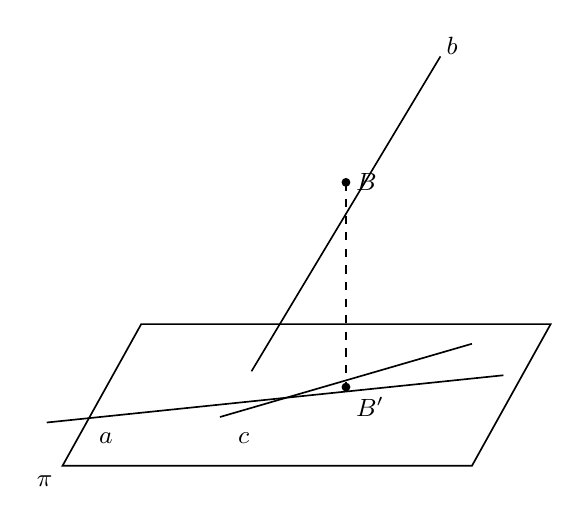
\begin{tikzpicture}[semithick, font=\small]
  % 平面 π
  \draw (0,0) -- (5.2,0) -- (6.2,1.8) -- (1.0,1.8) -- cycle;
  \node[below left] at (0,0) {$\pi$};
  % 直线 a（在平面内）
  \draw (-0.2,0.55) -- (5.6,1.15);
  \node[below] at (0.55,0.55) {$a$};
  % 投影 c（在平面内）
  \coordinate (B) at (3.6,3.6);
  \coordinate (Bp) at (3.6,1.0);
  \draw (2.0,0.62) -- (5.2,1.55);
  \node[below] at (2.3,0.55) {$c$};
  % 直线 b 及垂线 BB'
  \draw (2.4,1.2) -- (4.8,5.2);
  \node[above right] at (4.75,5.1) {$b$};
  \draw[dashed] (B) -- (Bp);
  \fill (Bp) circle (1.6pt);
  \node[below right] at (Bp) {$B'$};
  \fill (B) circle (1.6pt);
  \node[right] at (B) {$B$};
\end{tikzpicture}
\end{center}
\nopagebreak[4]
\Needspace{4\baselineskip}
\textbf{解析}
\Needspace{5\baselineskip}
\textbf{（1）} 设 $B$ 为直线 $b$ 上一点，$B'$ 为其在平面 $\pi$ 上的射影，则 $BB'\perp\pi$，$B'$ 在 $c$ 上。因为 $a\subset\pi$，所以 $a\perp BB'$。又 $a\perp b$，而 $b$，$BB'$ 是平面 $BB'c$ 内两条相交直线，故
\nopagebreak[4]
\[a\perp\text{\text{平面} }BB'c,\]
从而 $a\perp c$。

\textbf{（2）} 逆命题：若 $a\perp c$，则 $a\perp b$。

由 $a\perp c$ 及 $a\perp BB'$ 得 $a\perp$ 平面 $BB'c$，而 $b$ 在该平面内，故 $a\perp b$。逆命题为真。

\gkanswer{答案（1）：证明见解析。}

\gkanswer{答案（2）：逆命题为“若 $a\perp c$，则 $a\perp b$”，是真命题。}

\end{answer}
\begin{answer}
\gksolhead{19}{}

\textbf{题目}：

已知椭圆 $C_1:\dfrac{x^2}4+y^2=1$，椭圆 $C_2$ 以 $C_1$ 的长轴为短轴，且与 $C_1$ 有相同的离心率。

（1） 求椭圆 $C_2$ 的方程；

（2） 设 $O$ 为坐标原点，点 $A$，$B$ 分别在椭圆 $C_1$ 和 $C_2$ 上，$\overrightarrow{OB}=2\overrightarrow{OA}$，求直线 $AB$ 的方程。

\Needspace{4\baselineskip}
\textbf{解析}
\Needspace{5\baselineskip}
\textbf{（1）} $C_1$ 中 $a=2$，$b=1$，$e=\dfrac{\sqrt3}2$。$C_2$ 以 $C_1$ 的长轴为短轴，故短半轴为 $2$；离心率相同，得长半轴为 $4$，长轴沿 $y$ 轴：
\nopagebreak[4]
\[\frac{x^2}4+\frac{y^2}{16}=1.\]

\Needspace{5\baselineskip}
\textbf{（2）} 设 $A(x,y)$，由 $\overrightarrow{OB}=2\overrightarrow{OA}$ 得 $B(2x,2y)$。$B$ 在 $C_2$ 上：
\nopagebreak[4]
\[\frac{4x^2}4+\frac{4y^2}{16}=x^2+\frac{y^2}4=1.\]
与 $\dfrac{x^2}4+y^2=1$ 相减得 $\dfrac34x^2-\dfrac34y^2=0$，即 $y=\pm x$。故直线 $AB$ 的方程为 $y=x$ 或 $y=-x$。

\gkanswer{答案（1）：$\dfrac{x^2}4+\dfrac{y^2}{16}=1$。}

\gkanswer{答案（2）：$y=x$ 或 $y=-x$。}

\end{answer}
\begin{answer}
\gksolhead{20}{}

\textbf{题目}：

某银行柜台设有一个服务窗口，假设顾客办理业务所需的时间互相独立，且都是整数分钟，对以往顾客办理业务所需的时间统计结果如下：

\begin{center}
\begin{tabular}{llllll}
\toprule
办理业务所需的时间（分） & $1$ & $2$ & $3$ & $4$ & $5$ \\
\midrule
频率 & $0.1$ & $0.4$ & $0.3$ & $0.1$ & $0.1$ \\
\bottomrule
\end{tabular}
\end{center}

从第一个顾客开始办理业务时计时。

（1） 估计第三个顾客恰好等待 $4$ 分钟开始办理业务的概率；

（2） $X$ 表示至第 $2$ 分钟末已办理完业务的顾客人数，求 $X$ 的分布列及数学期望。

\Needspace{4\baselineskip}
\textbf{解析}
\Needspace{5\baselineskip}
\textbf{（1）} 第三个顾客恰好等待 $4$ 分钟，即前两位顾客办理时间之和为 $4$ 分钟：
\nopagebreak[4]
\[P=0.1\times0.3+0.4\times0.4+0.3\times0.1=0.03+0.16+0.03=0.22.\]

\textbf{（2）} $X$ 的可能取值为 $0,1,2$。

$X=2$ 需前两位各用 $1$ 分钟：$P(X=2)=0.1\times0.1=0.01$。

\Needspace{5\baselineskip}
$X=1$ 有两种情形：第一位用 $1$ 分钟且第二位用时不少于 $2$ 分钟，或第一位恰用 $2$ 分钟：
\nopagebreak[4]
\[P(X=1)=0.1\times(1-0.1)+0.4=0.09+0.4=0.49.\]

故 $P(X=0)=1-0.01-0.49=0.5$。分布列为

\begin{center}
\begin{tabular}{llll}
\toprule
$X$ & $0$ & $1$ & $2$ \\
\midrule
$P$ & $0.5$ & $0.49$ & $0.01$ \\
\bottomrule
\end{tabular}
\end{center}

\nopagebreak[4]
\[EX=0\times0.5+1\times0.49+2\times0.01=0.51.\]

\gkanswer{答案（1）：$0.22$。}

\gkanswer{答案（2）：$P(X=0)=0.5$，$P(X=1)=0.49$，$P(X=2)=0.01$；$EX=0.51$。}

\end{answer}
\begin{answer}
\gksolhead{21}{}

\textbf{题目}：

设函数 $f_n(x)=x^n+bx+c$（$n\in\mathbf N_+$，$b$，$c\in\mathbf R$）。

（1） 设 $n\geqslant2$，$b=1$，$c=-1$，证明：$f_n(x)$ 在区间 $\left(\dfrac12,1\right)$ 内存在唯一零点；

（2） 设 $n=2$，若对任意 $x_1$，$x_2\in[-1,1]$，有 $|f_2(x_1)-f_2(x_2)|\leqslant4$，求 $b$ 的取值范围；

（3） 在（1）的条件下，设 $x_n$ 是 $f_n(x)$ 在 $\left(\dfrac12,1\right)$ 内的零点，判断数列 $x_2$，$x_3$，$\cdots$，$x_n$，$\cdots$ 的增减性。

\Needspace{4\baselineskip}
\textbf{解析}
\Needspace{5\baselineskip}
\textbf{（1）} $b=1$，$c=-1$ 时 $f_n(x)=x^n+x-1$，在 $\left(\dfrac12,1\right)$ 上 $f_n'(x)=nx^{n-1}+1>0$，故单调递增。又
\nopagebreak[4]
\[f_n\left(\frac12\right)=\frac1{2^n}-\frac12<0,\qquad f_n(1)=1>0,\]
由零点定理，在 $\left(\dfrac12,1\right)$ 内存在唯一零点。

\textbf{（2）} $f_2(x)=x^2+bx+c$，条件等价于 $f_2$ 在 $[-1,1]$ 上的最大值与最小值之差不超过 $4$。

\Needspace{5\baselineskip}
若 $|b|\leqslant2$，顶点 $x=-\dfrac b2$ 在区间内，最大值为 $\max\{f(-1),f(1)\}=1+c+|b|$，最小值为 $c-\dfrac{b^2}4$，故
\nopagebreak[4]
\[1+|b|+\frac{b^2}4\leqslant4,\]
即 $|b|^2+4|b|-12\leqslant0$，解得 $|b|\leqslant2$。

若 $|b|>2$，$f_2$ 在 $[-1,1]$ 上单调，差为 $|f(1)-f(-1)|=2|b|>4$，不满足。

故 $b\in[-2,2]$。

\Needspace{5\baselineskip}
\textbf{（3）} 由 $x_n^n+x_n-1=0$ 得 $x_n^n=1-x_n$。因 $x_n\in\left(\dfrac12,1\right)$，有 $x_n^{n+1}<x_n^n$，故
\nopagebreak[4]
\[f_{n+1}(x_n)=x_n^{n+1}+x_n-1<x_n^n+x_n-1=0=f_{n+1}(x_{n+1}).\]
$f_{n+1}$ 单调递增，故 $x_n<x_{n+1}$，即 $\{x_n\}$ 是递增数列。

\gkanswer{答案（1）：证明见解析。}

\gkanswer{答案（2）：$[-2,2]$。}

\gkanswer{答案（3）：$\{x_n\}$ 是递增数列。}

\end{answer}